% \pagebreak[4]
% \hspace*{1cm}
% \pagebreak[4]
% \hspace*{1cm}
% \pagebreak[4]
%\usepackage[round,colon,authoryear]{natbib}

\chapter{Kingdom-wide discovery of bacterial intrinsic termination motifs}
\label{sec:chapterPingpong}
\ifpdf
    \graphicspath{{Chapter5/Chapter5Figs/EPS/}{Chapter5/Chapter5Figs/}}
\fi

\section{Introduction}

As discussed in the previous chapter, intrinsic termination of transcription is a fundamental cellular process in many, if not all, bacterial species. As reviewed in the previous chapter, the bulk of work on intrinsic termination has focused on canonical Rho-independent terminators (RITs), consisting of a G/C-rich hairpin structure followed by a poly-U tail. This is due to both their prevalence in model organisms such as \textit{Escherichia coli} and \textit{Bacillus subtilis}, as well as the distinctiveness of this motif making it an easy target for automated classification.

Despite this focus on canonical RITs, a number of intrinsic terminators which do not rely on a poly-U tail for termination activity are known. These include synthetic constructs derived from canonical RITs \parencite{Abe1996}, as well as naturally occurring terminators in \textit{Streptomyces} \parencite{Deng1987, Neal1991, Ingham1995} and \textit{Mycobacteria} \parencite{Unniraman2001}. Additionally, a number of ncRNA screens in Actinobacteria have described potential non-canonical RITs terminating ncRNA transcription \parencite{Swiercz2008,Miotto2012, Li2013}.  However, a more wide-spread effort at characterization of these elements has been hampered by two factors: their occurrence primarily in non-model organisms such as the Actinobacteria, and a lack of a systematic classification of these elements making it difficult to determine how wide-spread such elements are. The only study surveying potential alternative intrinsic terminators in the bacterial kingdom relied primarily on categorizing elements based on the shape of their predicted secondary structure \parencite{Unniraman2002}. However, this fails to consider the large number of very different sequences that can give rise to any particular secondary structure \parencite{Schuster1994}. It is well understood from studies of synthetic perturbations of canonical RITs that the sequence of both the hairpin structure and flanking sequence can have large, and often unexpected, effects on termination efficiency \parencite{Reynolds1992, Abe1996, Cambray2013, Chen2013}; there is no reason to think that non-canonical RITs would not exhibit a similar pattern of sequence specificity. As a result, there is a need for a robust classification of potential non-canonical RITs which considers both the sequence and structural features of these elements so that they can be systematically investigated. 

%Our view of bacterial diversity is expanding rapidly, particularly through the targeted sequencing of under-explored regions of the phylogeny \parencite{Wu2009} and recent advances in single-cell genomics enabling the sequencing of uncultivated organisms \parencite{Marcy2007, Rinke2013}, 

In the previous chapter I showed that covariance models (CMs) are able to capture sequence as well as structural features of canonical as well as putative non-canonical RITs. In this chapter I describe a method for the discovery of potential structured termination motifs across the bacterial kingdom, present an initial analysis of the elements discovered, and provide evidence for their activity through the analysis of a large collection of publicly-available RNA-seq data.

\section{Methods}

\textit{James Hadfield (University of Canterbury) ran the MCL clustering under my supervision. Paul P. Gardner (University of Canterbury) developed and ran the analysis of expression data, and assisted in manual curation of cluster alignments. Stinus Lindgreen (University of Canterbury/University of Copenhagen) processed RNA-seq data and performed mapping. I performed all other work described here. }

\subsection{Genome-wise motif discovery}
1853 EMBL format files containing the genomic sequence and annotations for 1639 bacteria were obtained from the EMBL European Nucleotide Archive completed bacterial genomes pages, {\color{red} NEED APPENDIX} information for organisms and accession numbers.

Each EMBL file was screened independently for putative multi-copy termination motifs. For each EMBL file, I extracted sequences from -20 to +80 around annotated ORF\nomenclature[Z]{ORF}{Open reading frame} stop site. Each extracted sequence was screened for a lower than expected predicted MFE using RNAfold in order to screen out locally GC-rich but unstructured sequences. The sequence under consideration was shuffled 1000 times preserving dinucleotide frequencies, and a Gumbel distribution was fitted to the resulting empirical null MFE distribution using the R MASS package \parencite{Venables1994}. Sequences with a native MFE below the 95th percentile of the null distribution were discarded. The resulting set of sequences was then given as input to CMfinder \parencite{Yao2006}, which produces collections of locally-aligned structurally conserved motifs. I built a CM for each motif using Infernal 1.0.2 \parencite{Nawrocki2009}.  The resulting CMs were searched against the EMBL file the motif was discovered in, and were then screened on the following criteria for the collection of search hits with an E-value of less than 1: a copy number of between 100 and 3000, and a median distance of $<$10 to the nearest annotated ORF stop site. This resulted in a collection of 4359 putative termination motif CMs, each derived from a single EMBL file. 

\subsection{Clustering covariance models}

In order to cluster CMs, I developed an extension of MCL-based clustering \parencite{Enright2002} to generative models of sequence variation. I call the measure of CM similarity I developed for this purpose the reciprocal similarity score (RSS), defined as: \[ \left[\frac{\sum_{i=1}^{n} -\ln{(E_{x,y,i})} +  \sum_{j=1}^{n} -\ln{(E_{x,y,j})}}{2n}\right] + \ln(n) \] where $E_{x,y,i}$ is the E-value of the $i$th sequence emitted by model $x$ scored by model $y$ and for the purposes of this study $n=1000$. Briefly, for each pair of CMs 1000 sequences were emitted from each CM and reciprocally scored with the other CM. The average of the negative log-transformed E-values was calculated, then shifted to be strictly positive by adding $\ln(1000)$ to generate the RSS\nomenclature[Z]{RSS}{Reciprocal similarity score} appropriate for use with MCL. MCL was run over the resulting RSS matrix, and the 100 largest clusters, ranging in size from 332 to 6 CMs, were taken forward for further analysis.

\subsection{Building consensus covariance models}

To build covariance models which captured the diversity of sequences represented by each cluster, I searched the ten CMs with the highest sum of RSS scores in each cluster against the set of genomes which contributed motifs to the cluster. Sequences on which at least four CMs agreed on with an E-value of $<$ 1 were collected. The redundancy of the collected sequences was iteratively reduced in an alignment-free fashion using cd-hit \parencite{Li2006} with the parameters -G 0 -aL 0.1 -aS 0.3 until there were less than 2000 sequences remaining or there were no remaining sequences with $>$ 85\% nucleotide identity. Sequences were extended by 20 bases on each side to capture features which may not have been in the CMfinder-derived motifs, e.g. poorly conserved poly-U tracts. The resulting set of sequences was aligned using MAFFT Q-INS-i \parencite{Katoh2008} using McCaskill base-pairing probabilities \parencite{McCaskill1990}, and secondary structures were predicted using CentroidAlifold \parencite{Hamada2009}, again with McCaskill base-pairing probabilities. CMs were built from the resulting cluster alignments, and sequences which did not match the CM with a bitscore of at least 20 were iteratively discarded. The resulting alignments were then manually curated using RALEE \parencite{Griffiths-Jones2005}, trimming non-conserved flanking sequence and extending the predicted secondary structure where possible. Conserved stop codons were specifically trimmed, so as not to bias subsequent searches.

\subsection{Genome annotation}

The resulting cluster CMs were searched over the initial 1853 EMBL files. Bitscore thresholds were set for hit significance for each cluster CM using shuffled sequence. Specifically, each cluster model was also used to search a dinucleotide shuffled database of these same 1853 EMBL file. For each model, a Gumbel distribution was fitted to the distribution of bitscores over the shuffled database, and this null Gumbel distribution was used to compute P-values for hit significance in the native sequences. P-values were corrected for multiple hypothesis testing using the method of \textcite{Benjamini1995}, and these were used to set bitscore thresholds at specific FDRs.

\subsection{Analysis of expression data}

Data sets were downloaded from the SRA \parencite{Leinonen2011}, preferring whenever possible to start our own analyses with the raw fastq input instead of relying on previous mapping results. This was done to make the data sets comparable. After retrieving the data sets, we extracted fastq reads for further analysis. Most data sets were downloaded in SRA format. Fastq files were extracted using the command �fastqdump --split-3� from the SRA toolkit version 2.3.2-4. This creates two fastq files in the case of paired end data, and one fastq file in case of single end data. When BED files were used as the primary input, the BAM file was extracted directly using �bedToBam� from the bedtools package, version 2.17.0 \parencite{Quinlan2010}. Data sets in SOLiD format was translated to fastq using �solid2fastq� from bfast version 0.7.0a \parencite{Homer2009}. All extracted fastq files were cleaned using AdapterRemoval version 1.4 \parencite{Lindgreen2012} with the flags �--trimns --trimqualities � to remove residual adapters from the reads and to remove low quality segments and stretches of Ns in the 5� and/or 3� ends.

Most data sets were mapped using bowtie2 version 2.1 \parencite{Langmead2012}, and the output was saved in BAM format using samtools version 0.1.18 \parencite{Li2009}. In the single end case, the following command was used:
\begin{verbatim} 
bowtie2 -x <INDEX> -U <READS> |samtools view -bS - \
| samtools sort - <OUTPUT>.sorted
\end{verbatim}

In the paired end case, a similar command was used, but the number of input files was larger because 1) there are two files containing the paired reads, and 2) additional single end reads might have been produced by AdapterRemoval because some pairs were collapsed due to overlaps, or one mate pair was discarded due to e.g. low quality. For 454 data, using the above command produced few mappings to the reference genome. We therefore used bowtie2 but with relaxed parameters to accommodate the longer reads by adding the flags �--local --very-sensitive-local�. For SOLiD data, we used bfast version 0.7.0a for mapping with the following commands:
\begin{verbatim}
bfast match -f <INDEX> -A 1 -r <READS> > <OUTPUT>.bmf
bfast localalign -f <INDEX> -A 1 -m <OUTPUT>.bmf > <OUTPUT>.baf
bfast postprocess -f <INDEX> -i <OUTPUT>.baf -A 1 | samtools view -bS - \
| samtools sort - <OUTPUT>.sorted
\end{verbatim}

For each BAM-file, we generated a PLOT file containing two tab separated columns (reverse strand, forward strand) and a line per position in the genome. Each line gives information on the number of mapped reads on each strand for that particular position in the reference genome. The PLOT files were generated using the following commands from samtools version 0.1.18:
\begin{verbatim}
samtools view -F 0x10 -b <INPUT> (for reads mapped to the forward strand)
samtools view -f 0x10 -b <INPUT> (for reads mapped to the reverse strand)
\end{verbatim}
Then, the �samtools depth� command was used to get the actual depths and save them in a WIG format file, which was then transformed to PLOT file by filling out the 0-depth positions based on the length of the reference genome.

Terminator activity plots were produced by selecting all predicted putative attenuation motifs (PAMs) with an upstream mean read count of at least 10. The median expression at each position between -80 and +80 with respect to the PAM was calculated and plotted. As a negative control, random positions meeting the criteria of a mean upsteam read count $\geq$ 10 were selected at random and their median recounts plotted. Specific data sets are cited in the text.

\section{Results}

\subsection{Kingdom-wide motif discovery}

The pipeline I developed for discovering putative termination motifs consisted of 3 major stages: genome-wise motif discovery with CMfinder  \parencite{Yao2006}, clustering of motifs using a novel similarity measure and the MCL algorithm \parencite{Enright2002}, and manual curation of the resulting motif clusters.  

In the first stage I extracted sequence from -20 to +80 with respect to annotated stop sites, which were then filtered on predicted structural potential to screen for sequences with stronger structures than predicted by their dinucleotide content alone (see Methods). For each genome, I used the resulting set of sequences as input for the CMfinder alogrithm \parencite{Yao2006}. Briefly, CMfinder uses heuristic sequence search, thermodynamic and mutual information-based predictions of secondary structure, and CM-based searches within an expectation-maximization (EM\nomenclature[Z]{EM}{Expectation-maximization}) framework to iteratively discover and refine potential structured RNA motifs, returning a multiple sequence alignment and corresponding CM. CMfinder has previously been successfully used as part of pipelines for the discovery of non-coding RNAs in bacteria \parencite{Weinberg2007, Weinberg2010} and eukaryotes \parencite{Torarinsson2008a}, as well as in our previous discovery of the TRIT element \parencite{Gardner2011a}. Applying this algorithm to the filtered sequences for each genome resulted in a total of 22310 motif predictions. I searched these CMs back over the genome they were predicted from and removed from consideration motifs with very low ($<$100) or very high ($>3000$) copy number, or were not enriched with respect to gene terminal regions, leaving a set of 4359 putative termination motifs, approximately 2.5 per organism.

To reduce the complexity of this data set, I developed a method for clustering CMs. Two previous approaches to comparing CMs have been described in the literature. The first, known as CMcompare \parencite{Honer-zu-Siederdissen2010}, computes the score of a so-called `link sequence', that is a sequence with the highest value of $\min{(S_1(s), S_2(s))}$, where $S_x(s)$ is the score of sequence $s$ with respect to model $S_x$. While this has been proposed as a measure of CM specificity in the context of the Rfam database, it is unclear how accurately this single link sequence captures the overlap between the sequence spaces described by two CMs, let alone the reality of overlaps in actual biological sequence databases. A second method, proposed as part of the Evofam pipeline for automated ncRNA family discovery in eukaryotic genome alignments \parencite{Parker2011}, approximates the Kullback-Leibler divergence between two CMs, that is the (dis)similarity of the probability distributions over sequences emitted by the two CMs, using the difference in Infernal CM E-value calculations on a human reference sequence from each model's training set. In the context of the Evofam pipeline, the use of the human reference sequence is justifiable, as the study was primarily concerned with the discovery of ncRNA families present in the human genome. However, in the present case of clustering motifs across an entire domain of life, there is no obvious single sequence to use as a reference for the purposes of a comparison between every pair of CMs.

\begin{figure}[htp]
\begin{center}
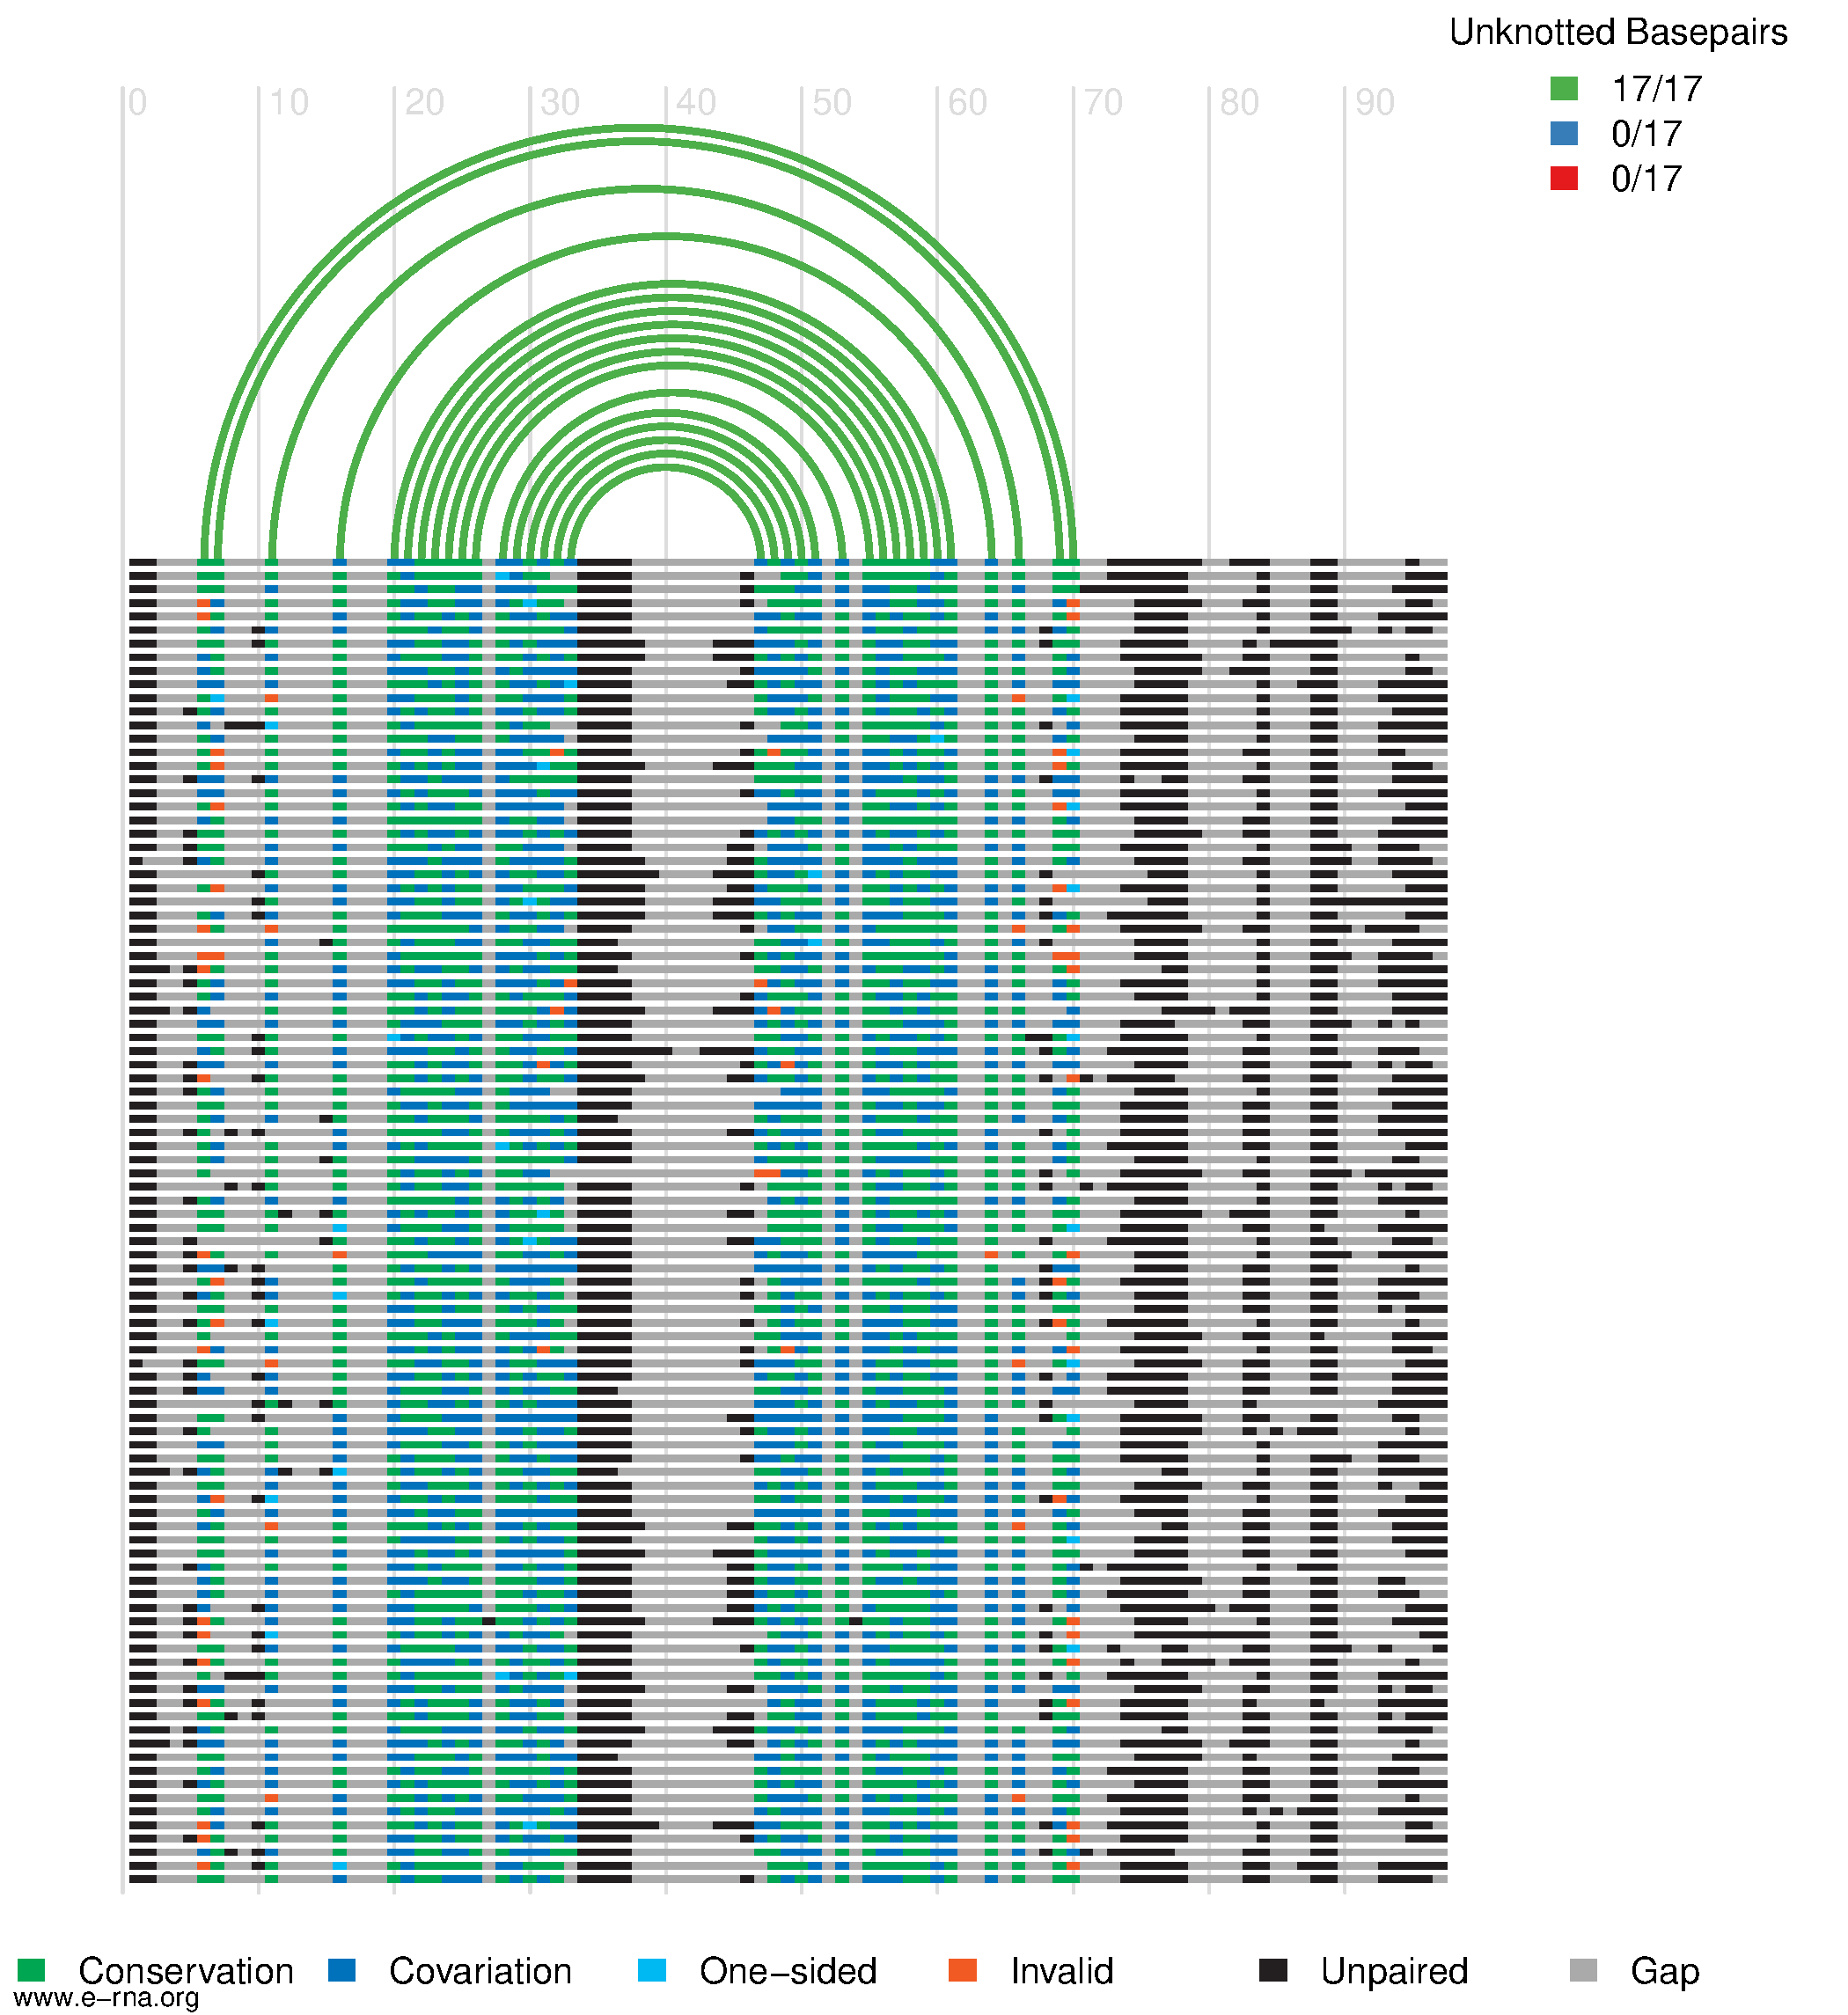
\includegraphics[width=14cm]{16_aln}
\caption[Example alignment of cluster consensus sequences]{\textbf{Example alignment of cluster consensus sequences.} Partial alignment of the consensus sequences for cluster 16, visualized using the R-CHIE webserver \parencite{Lai2012}. Green arcs represent base-pairing interactions. Nucleotides are visualized as blocks below, and are colored to highlight conservation and covariation in base-pairing relationships within the stem-loop structure.
} 
\label{fig:aln}
\end{center}
\end{figure}

I have developed a sampling based approach to measuring CM similarity, inspired by discussions of using summed bitscores as a measure of remote homology between CMs (personal communication, Paul P. Gardner and Sean R. Eddy) and the reciprocal BLAST measure used by TRIBE-MCL \parencite{Enright2002}. Rather than using a single reference sequence for the purpose of comparison, I use the fact that CMs are generative models to measure the average similarity of of their respective sequence spaces. Infernal reports bitscores and E-value for each match between a CM and a given sequence region. The bitscore, ignoring the specifics of algorithm used (either CYK or Inside), is \[S = \log_2\left({\frac{P(x \mid H)}{P(x \mid R)}}\right)\] where $P(x \mid H)$ is the probability of sequence $x$ under model $H$, and $P(x \mid R)$ is the probability of $x$ under a null model $R$, generally an iid\nomenclature[Z]{iid}{Independent identically distributed (random variable)} sites model with a geometric length distribution. This score is expected to follow a Type 1 Extreme Value (or Gumbel) distribution \parencite{Karlin1990, Eddy2008}, and this empirically appears to be the case for Infernal scores \parencite{Nawrocki2007}. Hence the E-value can be calculated as \[e^{-\lambda(S - \mu)}\] where $\lambda$ and $\mu$ are fitted parameters depending on the size of the database searched and the model architecture, and normalize for these factors. So the reciprocal similarity score (RSS) I have defined: \[ RSS_{x,y} = \left[\frac{\sum_{i=1}^{n} -\ln{(E_{x,y,i})} +  \sum_{j=1}^{n} -\ln{(E_{y,x,j})}}{2n}\right] + \ln(n) \] where $E_{x,y,i}$ is the E-value of the $i$th sequence emitted by model $x$ scored by model $y$, can be understood as the average normalized bitscore of each model over the other's sequence space, and is similar in spirit to Monte Carlo approximations to the Kullback-Leibler divergence \parencite{Parker2011,Juang1985}. 

This measure appeared robust to the number of samples used, but this may depend in part on model complexity. As the maximal E-value in this case is $n$, $-\ln(n)$ is a theoretical lower bound on the average $-\ln{(E)}$, and the subtraction of this factor ensures that the RSS is strictly positive. It is worth noting that this measure is symmetric ignoring sampling error. Asymmetric variants may have some applications. For instance, by taking the minimum of the average bitscore under either model, one would give preference to full-length model matches in comparisons between models of various sizes due to the glocal nature of Infernal search (global with respect to the model, local with respect to sequence), and this may be preferable for determining similarity between ncRNA families. Conversely, taking the maximum may have some utility in searching for shorter motifs. In the current application, I expect all CMs to be of roughly similar sizes and symmetric measures simplify clustering. This measure should be applicable to any generative model, and so could be similarly used to cluster e.g. HMMs.

A related measure was previously used by the TRIBE-MCL algorithm to cluster protein families based on reciprocal $\log_{10}$ BLAST E-values \parencite{Enright2002}. The MCL algorithm is described in detail elsewhere \parencite{VanDongen2008}, but in brief it uses simulations of random walks on a weighted graph to define clusters through an unsupervised, iterative process. Unsurprisingly, many of the clusters that were generated using MCL with RSSes appeared to be composed of CMs representing canonical RITs on visual inspection with some notable exceptions, described below. However, despite a complete lack of phylogenetic assumptions in our pipeline, we found that the majority of clusters were dominated by one or two orders, generally within the same phyla, and sometimes even a single genera. This both validates our clustering procedure and indicates that RITs, despite their small size and stereotypical sequence composition, carry a phylogenetic signal when considered in aggregate.

To further study lineage-specific biases in terminator composition, I took the top 100 clusters, ranging in size from 332 to 6 CMs, and constructed consensus models through a semi-automated process. First, for each cluster I selected the 10 CMs with the highest sum of RSS scores with other cluster CMs (or all CMs in the case of clusters with $<$ 10 members), and searched these across all of the genomes the cluster CMs were derived from. Regions that these CMs agreed were likely to be terminator sequences were collected and aligned using MAFFT Q-INS-i \parencite{Katoh2008}, a heuristic Sankoff alignment algorithm which considers both sequence and secondary structure in alignment, and secondary structure was predicted using CentroidAlifold \parencite{Hamada2009}, and manually refined using RALEE \parencite{Griffiths-Jones2005} (see figure \ref{fig:aln}; see also Methods for detailed alignment protocol). I annotated the 1853 EMBL files we started with, and iteratively removed from consideration any model with at least 85\% of its sequence hits covered by another model. This left 16 putative terminator models, on which all further analysis was done.



\subsection{Canonical RIT diversity}

\begin{figure}[htp]
\begin{center}
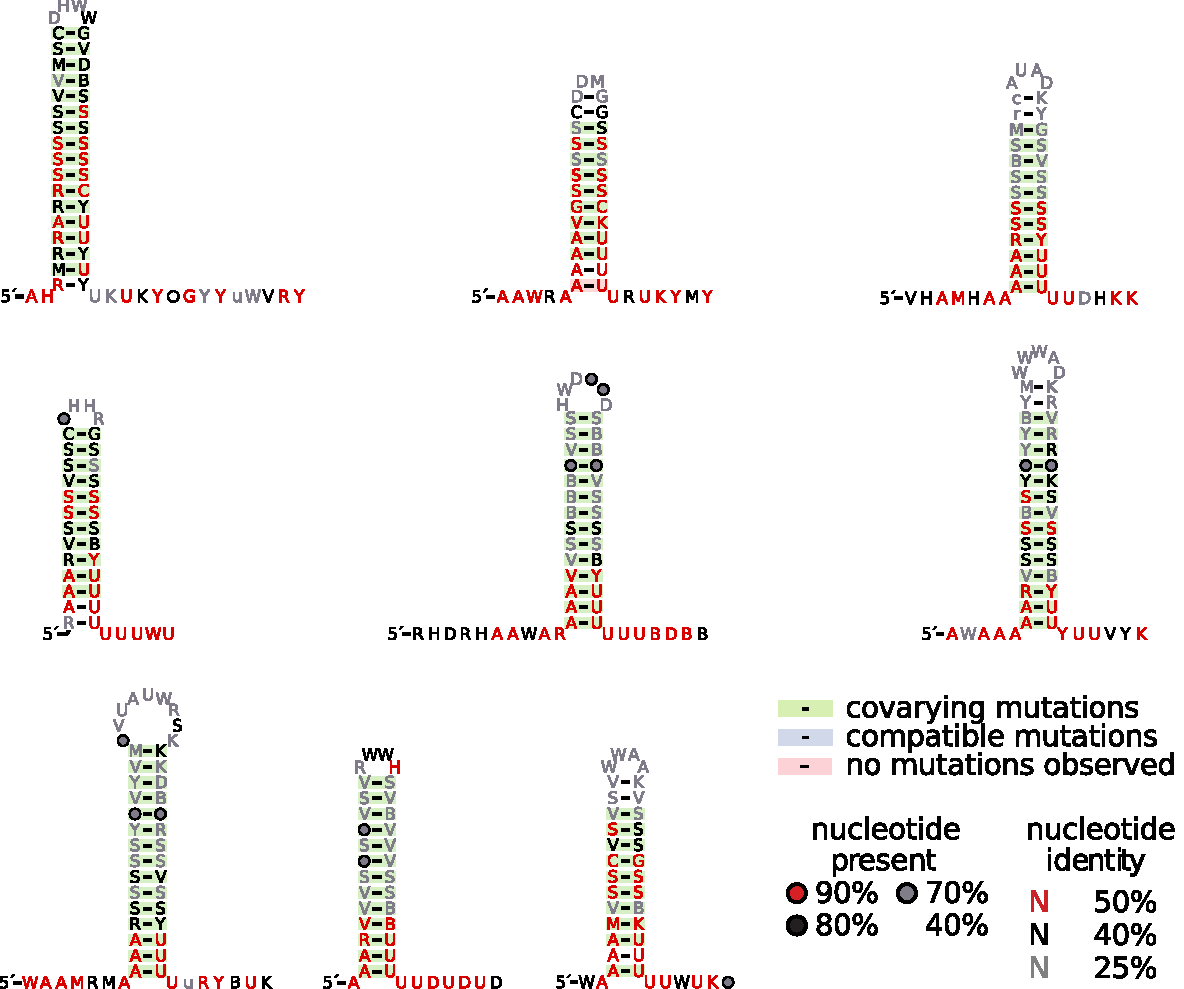
\includegraphics[width=14cm]{canonical}
\caption[Most informative sequences for nine canonical RIT clusters]{\textbf{Most informative sequence for nine canonical RIT clusters.} Each cluster consensus model was searched across all genomes and sequence hits with an FDR of 0.01 were aligned to the model. Duplicate sequences were removed and 5000 randomly sampled sequences were used to calculate the most informative sequence (MIS)\nomenclature[Z]{MIS}{Most informative sequence}, a projection of any bases with frequencies above .25 onto IUPAC characters \parencite{Freyhult2005}. Structures were drawn using R2R \parencite{Weinberg2011}. From left to right, images shown represent consensus alignments for clusters 16, 18, 25 (top row); 29, 37, 88 (middle row); 89, 95, and 96 (bottom row).
} 
\label{fig:canonical}
\end{center}
\end{figure}

Of the 16 resulting cluster, 9 appeared to be canonical RITs on visual inspection (see figure \ref{fig:canonical}). All shared known features of canonical RITs, including a $5^\prime$ poly-A region, a G/C-rich hairpin, and a poly-U tail, but differ in stem length, hairpin loop length, and base composition. An interesting feature of these models is the universal presence of base-pairing interactions between the poly-A and poly-U regions. Though it has been widely assumed that the poly-A region's function is primarily to contribute to bidirectional activity of RITs, some studies have shown that complementarity between the poly-A and poly-U region increase termination efficiency \parencite{Abe1996, Chen2013}, presumably by contributing to the ratcheting effect of hairpin formation on the poly-U tail. In fact, a recent study showed that strong terminators with clear poly-A regions generally do not posses strong bidirectional activity, suggesting that the primary function of the poly-A region is to contribute to this ratcheting \parencite{Chen2013}. I have observed covariation within many of the A-U pairs in our terminator models, supporting this observation.

\subsubsection{Validating RIT activity with RNA-seq}

To validate RIT predictions, publicly available RNA-seq datasets were collected and plots summarizing the behavior of transcription across the predictions were created (see Methods for details). There are some difficulties in using RNA-seq data to validate terminator activity. In perfect digital transcriptomic data, we would expect to observe the majority of transcripts terminating precisely within the poly-U tail of annotated RITs. Unfortunately, modern high-throughput sequencing technologies do not sequence complete RNA molecules, rather sequencing short stretches of size-selected fragmented RNA libraries. These fragments in these libraries are incidentally selected for sequence composition during both library amplification through PCR and sequencing, often with poorly understood biases, giving rise to the characteristically hilly appearance of these data sets when visualized. Additonally, protocols for the sequencing of RNA retaining strand information generally sequence all fragments of a particular RNA molecule in the same direction (for example, see \textcite{Croucher2009}). As a result, if we assume that the fragmentation proceeds roughly by a Poisson process, this will naturally lead to an exponential decay in apparent expression along the $3^\prime$ region of each transcript. Newer data sets with longer read lengths tend to give cleaner indications of termination activity. Finally, in some data sets we observed patterns of reported transcription that are suggestive of degradation of the RNA by $3^\prime$ exonucleases or high levels of genomic DNA contamination. 

\begin{figure}[htp]
\begin{center}
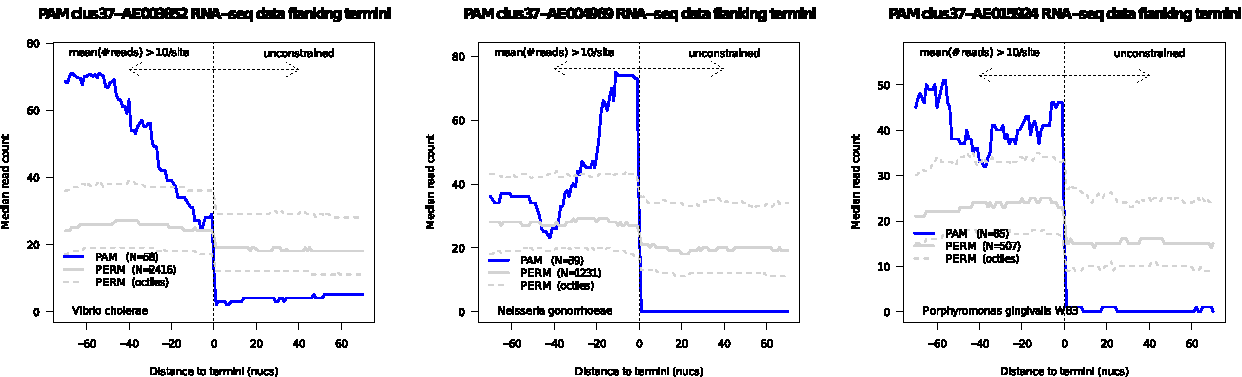
\includegraphics[width=16cm]{can_expr}
\caption[Analysis of diverse RNA-seq datasets confirm canonical terminator activity]{\textbf{Analysis of diverse RNA-seq datasets confirm canonical terminator activity.} These plots present representative analysis for putative attenuation motifs (PAM)\nomenclature[Z]{PAM}{Putative attenuation motif} predicted by the cluster 37 canonical terminator consensus model. The median expression over PAMs with an upstream mean expression of at least 10 reads per position is plotted in blue. Random positions meeting this same constraint are plotted in grey, and the dashed grey lines provide a 75\% confidence interval for this estimate. RNA-seq data (from left to right) drawn from experiments in the $\gamma$-proteobacterium \textit{Vibrio cholerae} \parencite{Mandlik2011}, the $\beta$-proteobacterium \textit{Neisseria gonorrhoeae} \parencite{Isabella2011}, and the Bacteroidetes \textit{Porphyromonas gingivalis} \parencite{Hovik2012}.
} 
\label{fig:can_expr}
\end{center}
\end{figure}

Despite these potential problems, when taken in aggregate, a clear signal from the termination activity of canonical RITs can be observed (see figure \ref{fig:can_expr} for examples). These plots present median read counts over predicted RITs as a robust estimator of the mean expression. As a control, the median read counts over randomly selected positions were similarly selected. A clear difference in the change in the level of transcription over RITs can be observed as compared to random positions, often much larger than the difference between the top estimate of a 75\% confidence interval before and the bottom estimate after these randomly positions. This pattern appears to hold for all of the canonical RIT clusters discovered in the course of this work. I did observe cases where there did not appear to be characteristic drop in transcription across predicted canonical RITs; however, these could generally be attributed to high levels of `background transcription' (possibly resulting from sample contamination with genomic DNA) confounding the selection criteria on element upstream transcription (see methods for details). An adaptive selection criteria based on the median absolute deviation from the median transcription across all positions in the genome, rather than an arbitrary cut-off on mean transcription, may correct this, and we are currently pursuing this possibility. As it stands, these plots provide a qualitative indication of termination activity. However, it should be possible to quantify these results using, e.g., a permutation test on the change in median transcription over random samples of the same size as the number of predicted RITs meeting the upstream transcription selection criterion.

\subsubsection{Lineage-specific enrichment of canonical RIT clusters}

\begin{figure}[htp]
\begin{center}
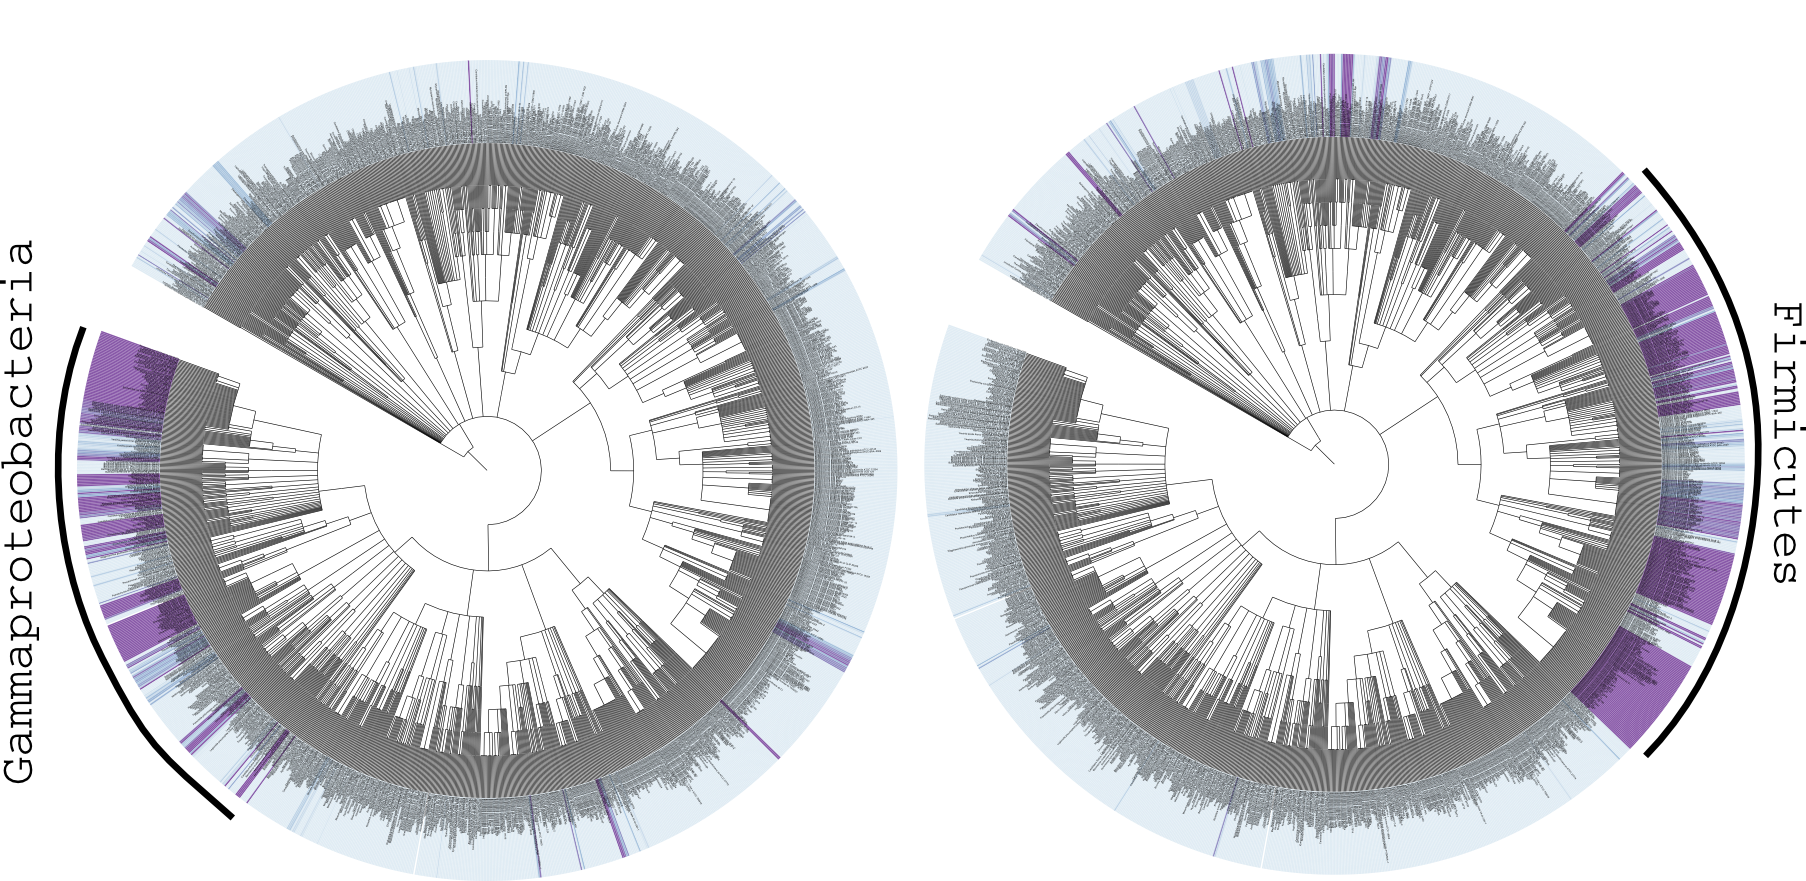
\includegraphics[width=16cm]{enrichment.png}
\caption[Canonical RIT enrichment on the NCBI taxonomy]{\textbf{Canonical RIT enrichment on the NCBI taxonomy.} These figures show the extent of canonical RIT enrichment in each genome for canonical RIT clusters 18 (left) and 37 (right). Each leaf node represents a single genome, and colors represent -$\log_{10}$ hypergeometric p-values ranging on a scale from light blue (no enrichment) to purple (high enrichment). Clades with large numbers of enriched genomes are annotated. Figures drawn using the Interactive Tree of Life webserver \parencite{Letunic2011}.
} 
\label{fig:enrichment}
\end{center}
\end{figure}

As noted previously, many of the clusters recovered by the motif-discovery pipeline appeared to consist largely of elements discovered in related genomes. The final consensus alignments constructed from these clusters have broadly similar architectures (see figure \ref{fig:canonical}), so it was unclear if they would retain the characteristics which allowed the RSS-based MCL clustering to recover the phylogenetic relationships between host genomes. To provide an initial assessment of the lineage-specificity of the motifs, I performed a hypergeometric test for element enrichment in each genome for each cluster. This revealed clear patterns of lineage-specific enrichment for each element (see figure \ref{fig:enrichment} for representative examples). 

Two alternative hypotheses could explain these patterns. The first, which I will term the global selection hypothesis, is selection for a particular form of terminator motif. This could be either active selection for robust terminator activity in the face of an evolving transcription apparatus \parencite{Iyer2004}, or an incidental effect of selection for other genomic properties such as G/C content, or more likely, a combination of both. The second, which I will call the transposition hypothesis, would be based on the distribution of particular RIT forms by transposable elements and would imply an evolutionary relationship between members of a particular RIT cluster. Transposable elements have previously been suggested as a means for the distribution of RITs later exapted as elements of $5^\prime$ cis-regulatory elements by \textcite{Naville2010}, and there is no reason a similar mechanism could not deposit $3^\prime$ RITs. Given the apparently ancient origins of many of the observed lineage-specific enrichments, the deposited RITs would subsequently have to be somewhat protected from random mutations preserving termination activity by a selective process, though as the degree of sequence and structural divergence allowed by the CM-based classification is currently unclear, this may well be possible. Of course, these two hypotheses are not mutually exclusive, and could act together to explain the observed pattern of terminator enrichment. It is important to note that enrichment of one RIT cluster does not imply the exclusion of alternative terminator structures in a particular genome. As seen in figure \ref{fig:can_expr} RIT clusters are present and apparently active outside the genomes they are enriched in; in this case, cluster 37, enriched primarily in the Firmicutes, is present at fairly low copy numbers in other phyla. Whether this reflects convergence or shared descent of these elements is unclear.

\subsection{Non-canonical putative attenuators of transcription}

Besides the canonical RITs discussed so far, the motif discovery pipeline uncovered 7 clusters which did not fit the canonical RIT model of a G/C-rich hairpin followed by a poly-U tract. I will refer to these elements as putative attenuators of transcription (PAMs). These elements tend to have much narrower host ranges than the canonical RITs discussed above; I discuss a few of them in the following sections.

\subsubsection{The Neisserial DNA uptake sequence PAM}

\begin{wrapfigure}{hr}{0.5\textwidth}
\begin{center}
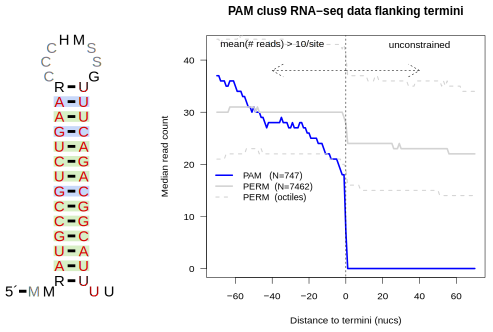
\includegraphics[width=7cm]{clus9}
\caption[Neisserial DNA uptake sequence terminator]{\textbf{Neisserial DNA uptake sequence terminator.} On the left, consensus secondary structure and MIS for 2012 non-identical cluster 9 PAMs in the order Neisseriales. On the right, median expression over predicted terminator sequences derived from RNA-seq experiments in \textit{Neisseria gonorrhoeae} \parencite{Isabella2011}.
} 
\label{fig:clus9}
\end{center}
\end{wrapfigure}

This first, and perhaps one of the most distinctive, of these elements is a previously known PAM containing a DNA uptake sequence (DUS\nomenclature[Z]{DUS}{DNA uptake sequence}) in the $\beta$-proteobacterial order Neisseriales. The Neisseriales frequently exchange genetic material, leading to difficulties in studying their population structure and so-called `fuzzy' species \parencite{Corander2012}. This exchange is mediated by specific systems \parencite{Hamilton2006}. Neisserial species are able to excrete DNA for donation through a type 4 secretion system and/or autolysis. A type 4 pilus-like system is then thought to specifically bind DNA containing a 10-base DUS (GCCGTCTGAA in \textit{Neisseria gonorrhoeae}), which is then incorporated in to the genome through homologous recombination. Recent work has shown that there are a number of distinct `dialects' of DUS which act to reduce the efficiency of uptake between distantly related species within the order \parencite{Frye2013}.

The presence of the \textit{Neisseria} DUS in terminator-like structures has long been noted \parencite{Goodman1988}, and was discussed extensively  in the study reporting the development of TransTermHP \parencite{Kingsford2007}. However, the termination activity of this element has never been experimentally tested. Using our RNA-seq collection, we are able to show that this element is indeed associated with a sharp drop in transcription (see figure \ref{fig:clus9}).

\subsubsection{The Actionbacterial PAM}

\begin{figure}[htp]
\begin{center}
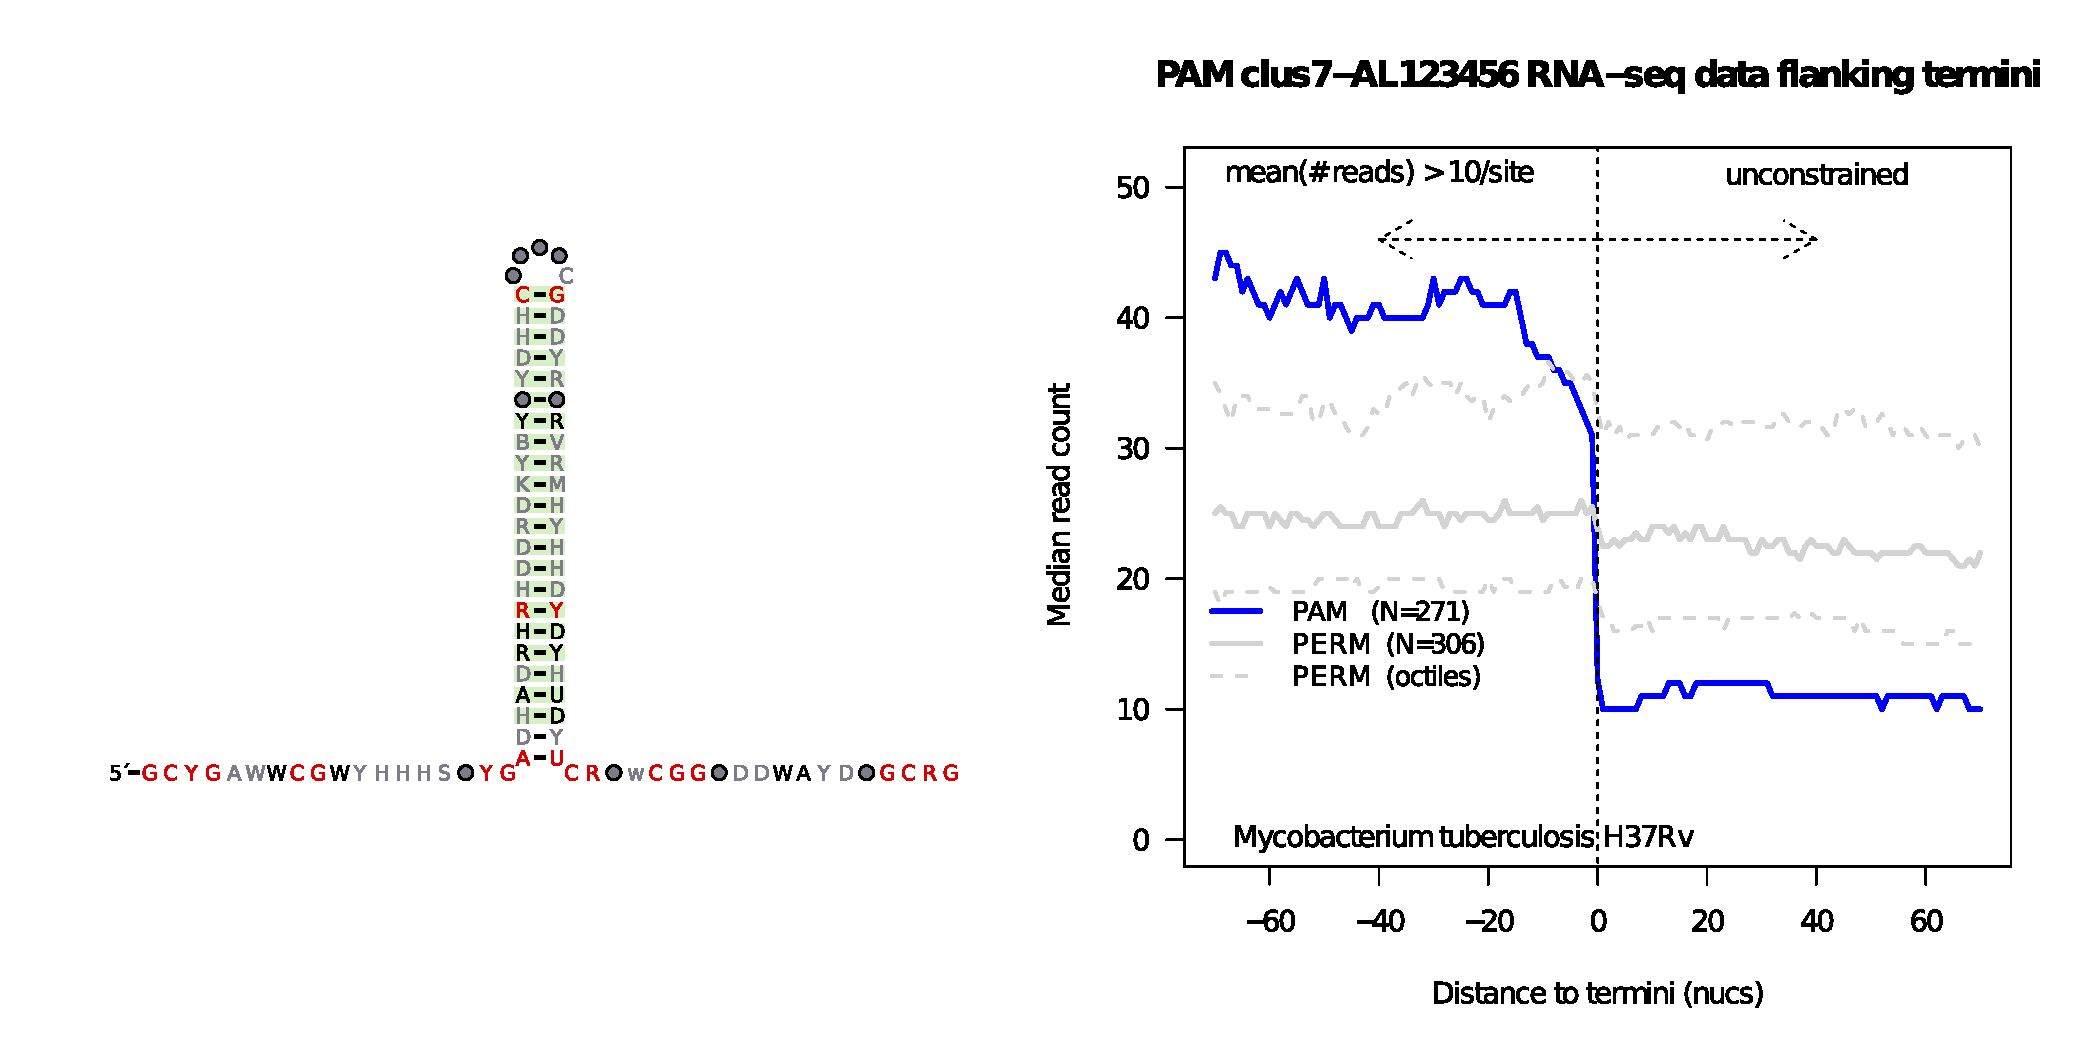
\includegraphics[width=14cm]{clus7}
\caption[Actinobacterial PAM]{\textbf{Actinobacterial PAM.} On the left, consensus secondary structure and MIS for 2891 non-identical cluster 7 PAMs in the class Actinobacteria. On the right, median expression over predicted terminator sequences derived from RNA-seq experiments in \textit{Mycobacterium tuberculosis} \parencite{Arnvig2011}.
} 
\label{fig:clus7}
\end{center}
\end{figure}

The motif discovery pipeline also recovered a motif redundant with the one previously dubbed TRIT in chapter 4 and \textcite{Gardner2011a}, cluster 7. The enrichment analysis I performed indicated that rather than being restricted to the \textit{Mycobacteria} as we previously hypothesized, this element appears to occur throughout the Actinobacteria. This motif also overlaps with two `I-shaped' elements previously discovered in an MFE-based screen for non-canonical termination motifs \parencite{Unniraman2001}, downstream of the \textit{Mycobacterium tuberculosis} genes \textit{tuf} and \textit{Rv1324}. These structures have previously been shown to reduce expression of downstream genes by $\sim$80\% in synthetic constructs \textit{in vivo} in \textit{Mycobacterium smegmatis}, and to specifically terminate transcription \textit{in vitro}. The results of our RNA-seq analysis (see figure \ref{fig:clus7}) suggest that this termination activity holds for the entire class of these elements.

Interestingly, the enrichment analysis also showed overrepresentation of hits in a number of Proteobacterial genera, including \textit{Pseudomonas} species. Analysis of RNA-seq data in \textit{Pseudomonas putida} \parencite{Frank2011}, which harbors $\sim$300 putative copies of this element, showed no evidence of involvement in transcription termination. An alignment generated from the putative \textit{Pseudomonas} sequences contained extended G/C-rich sequence within the loop region of the motif, which could potentially form an extended secondary structure. Together, this suggests that the \textit{Pseudomonas} element is not a member of the same class as the Actinobacterial element, and these hits may be a result of low specificity in the cluster consensus model, likely due to partial similarity between the stem structure of the two elements confounding the RSS measure. A second cluster with exclusively Actinobacterial sequences was also discovered by MCL, and it is possible this has higher specificity for the PAM. Alternatively, the specificity of the cluster 7 model could potentially be increased by removing non-Actinobacterial seqeunces from the alignment. 

\subsubsection{Type 1 integron attC sites}

\begin{wrapfigure}{hl}{0.5\textwidth}
\begin{center}
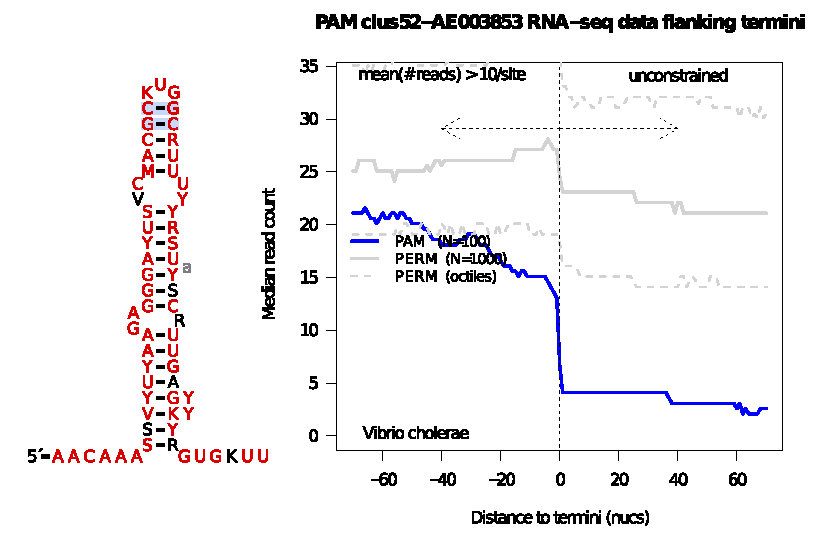
\includegraphics[width=7cm]{clus52}
\caption[Type 1 integron attC sites]{\textbf{Type 1 integron attC sites.} On the left, consensus secondary structure and MIS for 420 cluster 52 PAMs in the Proteobacteria. On the right, median expression over predicted terminator sequences derived from RNA-seq experiments in \textit{Vibrio cholerae} \parencite{Mandlik2011}.
} 
\label{fig:clus52}
\end{center}
\end{wrapfigure}

Many Gram-negative bacteria harbor arrays of horizontally-acquired gene cassettes known as integrons \parencite{Hall2012}. The architecture of these integrons is roughly similar, consisting of an \textit{intI} gene encoding an integrase, an \textit{attI} integration site, and a series of gene cassettes containing \textit{attC} sites important for recognition by IntI. While the sequence of \textit{attC} sites can vary widely, it has long been known that the \textit{attC} sites of the \textit{Vibrio cholerae} type 1 integron are unusually homogenous. My pipeline discovered this motif (see figure \ref{fig:clus52}), and it is enriched primarily in \textit{Vibrio} and \textit{Shewanella} genomes, though can be found sporadically at low copy number throughout the $\gamma$-proteobacteria. Expression of type 1 integrons is thought to be driven primarily by a single upstream promoter. An early study of this expression suggested that the \textit{attC} sites may be acting as transcriptional terminators based on Northern blots showing that transcripts did not cover the entire integron and tended to contain full-length gene cassettes, and that transcript frequency was inversely correlated with transcript length \parencite{Collis1995}. A single study has attempted verify this hypothesis, and found that \textit{attC} sites do not appear to promote transcriptional termination, and rather propose a mechanism for enhancing cassette expression through the presence of short ORFs within the \textit{attC} sites \parencite{Jacquier2009}. However, this study only tested a single \textit{attC} site with an atypically large hairpin-loop region for termination activity; additionally this study does not explain the patterns seen in the Northern blots of the \textcite{Collis1995} study. A recent study of the termination efficiency of a large number of transcriptional terminators included an \textit{attC} site in their initial screens, though it was discarded early in their study as being a low efficiency terminator \parencite{Cambray2013}. However, their initial experiments on this element, using a fluorescent reporter construct in \textit{Escherichia coli}, did show a termination efficiency of 25\%. Our analysis of RNA-seq data in \textit{Vibrio cholerae} appears to support the hypothesis that at least some \textit{attC} may operate as transcriptional attenuators. This stochastic attenuation at \textit{attC} sites would explain the results of \textcite{Collis1995}, and would lead to a gradual titration of expression along the length of integrons, barring the presence of internal promoters.

\subsubsection{Other non-canonical PAMs}

Four other non-canonical PAMs were identified by the motif-discovery pipeline. One of these appears to be a simple repeat family in the $\beta$-proteobacteria, and RNA-seq analysis indicates it is likely not involved in transcriptional termination. I am still investigating the potential activity of the other three at the time of writing.

\section{Discussion}

In a recent comprehensive review of transcriptional termination, \textcite{Peters2011} lay out four criteria for experimental validation of transcriptional terminators: 
\begin{quote}
1) it causes dissociation of (the elongation complex) during \textit{in vitro} transcription as detected by release of RNA and DNA from RNAP; 2) it generates terminated RNA $3^\prime$-ends before readthrough transcripts appear during synchronized \textit{in vitro} transcription; 3) it generates the terminated RNA $3^\prime$-ends \textit{in vivo}; and 4) it significantly reduces synthesis of RNA downstream from the site \textit{in vivo}.
\end{quote}

A primarily computational study as described here can not hope to meet this burden of evidence. Indeed, the authors of this review admit that only a small number of even canonical RITs have been subjected to this degree of validation, and furthermore discuss a number of cases where even ``obvious" RITs have turned out not to function as transcriptional terminators. However, while I can not rule out with certainty alternative explanations for the transcriptional patterns I have observed over predicted PAMs, such as protection from $3^\prime$ exonucleases, I believe that the evidence I have presented here in combination with previous studies suggesting possible non-canonical termination motifs is indicative of a wider diversity of intrinsic termination mechanisms than is immediately evident from studies in model organisms.

While the work presented here provides initial insights in to the diversity of elements associated with transcriptional termination, there remains a number of issues that need to be addressed in this study. Foremost is the criterion used to define the set of PAMs which I carried forward for enrichment and transcriptional analysis, that is $<$85\% overlap with all other PAMs across the phylogeny. It is well known that currently available genome sequences are highly biased towards a relatively small number of organisms that are easily cultivated; furthermore, this set is itself biased towards model species and human pathogens, which may not be representative of the phylogeny as a whole. It is possible that a more nuanced criterion, based for instance on overlaps at the class level, may provide a clearer picture of terminator diversity. Providing this view of terminator diversity will be increasingly important as our understanding of bacterial diversity expands in light of sequencing projects targeting underrepresented genera \parencite{Wu2009} and the difficult to cultivate `dark matter' of the phylogeny through single-cell sequencing \parencite{Marcy2007, Rinke2013}.

A second major challenge to be addressed is identifying the determinants which allow the CMs I have constructed to distinguish between classes of RITs in various lineages. These determinants may include the sequence compositions of particular regions or base-pairs within the terminator structure, or gross aspects of each class such as stem-length and G/C content. It is well known that the specific sequence composition of RITs can have large effects on termination efficiency in \textit{Escherichia coli}, even when maintaining the canonical G/C-rich hairpin followed by a poly-U tail \parencite{Chen2013, Cambray2013}. It seems likely that evolution of the transcriptional apparatus would change these design constraints, and I believe the methods I have developed in this study may allow us to begin to probe the parameters which may underlie RIT function in diverse host species.